% Minimal pandoc template for CQG (iopart.cls). Engine: xelatex (STIX Two Text).
\documentclass[12pt]{iopart}
\usepackage{iftex}
\ifPDFTeX
  \usepackage[T1]{fontenc}
  \usepackage[utf8]{inputenc}
\else
  \usepackage{fontspec}
  \setmainfont{STIX Two Text}
\fi
% iopart pre-defines \equation*; free it so amsmath can load cleanly, then iopams (amssymb+bold Greek)
\makeatletter
\expandafter\let\csname equation*\endcsname\relax
\expandafter\let\csname endequation*\endcsname\relax
\makeatother
\usepackage{amsmath}
\usepackage{iopams}
\usepackage[numbers,sort&compress]{natbib}   % iopart-num.bst is a natbib style
\usepackage{graphicx}
\usepackage[colorlinks=true,citecolor=blue,linkcolor=blue,urlcolor=blue]{hyperref}
\usepackage{orcidlink} % ORCID icon next to the author

% --- prose Unicode operators -> math ---
\usepackage{newunicodechar}
\newunicodechar{→}{\ensuremath{\rightarrow}}
\newunicodechar{∂}{\ensuremath{\partial}}
\newunicodechar{∈}{\ensuremath{\in}}
\newunicodechar{∎}{\ensuremath{\blacksquare}}
\newunicodechar{□}{\ensuremath{\Box}}
\newunicodechar{∝}{\ensuremath{\propto}}
\newunicodechar{∞}{\ensuremath{\infty}}
\newunicodechar{∫}{\ensuremath{\int}}
\newunicodechar{≈}{\ensuremath{\approx}}
\newunicodechar{≠}{\ensuremath{\neq}}
\newunicodechar{≡}{\ensuremath{\equiv}}
\newunicodechar{≤}{\ensuremath{\leq}}
\newunicodechar{≥}{\ensuremath{\geq}}
\newunicodechar{≪}{\ensuremath{\ll}}
\newunicodechar{≫}{\ensuremath{\gg}}
\newunicodechar{≲}{\ensuremath{\lesssim}}
\newunicodechar{⊙}{\ensuremath{\odot}}
\newunicodechar{⊗}{\ensuremath{\otimes}}
\newunicodechar{⟹}{\ensuremath{\Longrightarrow}}
\newunicodechar{⟺}{\ensuremath{\Longleftrightarrow}}
\newunicodechar{⇒}{\ensuremath{\Rightarrow}}
\newunicodechar{⇔}{\ensuremath{\Leftrightarrow}}
\newunicodechar{𝓗}{\ensuremath{\mathcal{H}}}
\newunicodechar{√}{\ensuremath{\surd}}
\newunicodechar{∼}{\ensuremath{\sim}}
\newunicodechar{∇}{\ensuremath{\nabla}}
\newunicodechar{↔}{\ensuremath{\leftrightarrow}}
\newunicodechar{⟨}{\ensuremath{\langle}}
\newunicodechar{⟩}{\ensuremath{\rangle}}
\newunicodechar{−}{\ensuremath{-}}
\newunicodechar{ℓ}{\ensuremath{\ell}}
\newunicodechar{ħ}{\ensuremath{\hbar}}
\newunicodechar{′}{\ensuremath{{}^\prime}}
\newunicodechar{Ḣ}{\ensuremath{\dot H}}
\newunicodechar{Ṡ}{\ensuremath{\dot S}}

% --- pandoc body requirements ---
\usepackage{longtable,booktabs,array}
\usepackage{calc}
\usepackage{float}
\makeatletter
\newsavebox\pandoc@box
\newcommand*\pandocbounded[1]{%
  \sbox\pandoc@box{#1}%
  \Gscale@div\@tempa{\textheight}{\dimexpr\ht\pandoc@box+\dp\pandoc@box\relax}%
  \Gscale@div\@tempb{\linewidth}{\wd\pandoc@box}%
  \ifdim\@tempb\p@<\@tempa\p@\let\@tempa\@tempb\fi%
  \ifdim\@tempa\p@<\p@\scalebox{\@tempa}{\usebox\pandoc@box}%
  \else\usebox{\pandoc@box}%
  \fi%
}
\makeatother
\providecommand{\tightlist}{\setlength{\itemsep}{0pt}\setlength{\parskip}{0pt}}
\graphicspath{{../../results/paper/}{../../results/}}

\setlength{\emergencystretch}{3em}


% --- make bibliography identifiers clickable -------------------------------
% Several bibliography styles (SciPost, iopart-num) emit \eprint{...} as plain
% text, leaving arXiv identifiers unclickable in the reference list. Redefine it
% to a hyperlink. Works for both new (2004.09444) and old (gr-qc/9504004) ids.
\providecommand{\eprint}[1]{#1}
\AtBeginDocument{\renewcommand{\eprint}[1]{\href{https://arxiv.org/abs/#1}{#1}}}

\begin{document}
% short running head (iopart overflows the page header with the full title)
\title[Barrow $\Delta \le 1$ from a long-range entanglement network]{Barrow
\(\Delta  \leq  1\) from a long-range entanglement network: a capacity
theorem and an area--volume dichotomy}
\author{Stilian Pandev\,\orcidlink{0009-0005-8153-071X}}
\address{Independent researcher}
\ead{stilianpandev@gmail.com}
\begin{abstract}We model the degrees of freedom of a gravitational
horizon as a network of Planck-density sites, each with a bounded total
entanglement weight \(\kappa\) (a finite local Hilbert-space dimension)
and bond weights decaying with separation as
\(w(r) \propto  r^{-\alpha }\). Three results follow. First, the
bond-cut capacity of any region \(\Omega\) obeys
\(C(\Omega ) \leq  \kappa\)\textbar{}\(\Omega\)\textbar, so the Barrow
entropy deformation satisfies \textbf{\(\Delta  \leq  1\) as a theorem}
of the model (the \emph{bound}; attaining \(\Delta  = 1\) additionally
needs the \(\alpha  < d\) volume-basin geometry --- derived here with an
explicit finite-size error bound, uniform in position --- and a
cut-saturating horizon \emph{state}, which we identify as the tracial
state of the site algebra, leaving open only whether a physical horizon
is driven to it) --- no fractal-horizon geometry is needed, and for
long-range couplings \((\alpha  < d)\) none is available, since the
minimum cut is not a surface. Second, the capacity is the enclosed
\emph{volume} \((\Delta  = 1)\) for every range \(\alpha  < d\) and the
boundary \emph{area} \((\Delta  = 0)\) for \(\alpha  > d + 1\);
gravity's Newtonian reach \((\alpha  = 1)\) lies deep in the volume
phase, and no gravitational coupling produces an intermediate range, so
a measured intermediate \(\Delta\) falsifies the picture rather than
selecting a parameter. Third, \(\Delta  = 1\) exactly is the
infrared-cutoff endpoint L → ∞ --- a stated choice, not a derivation.
What the network counts is a structural capacity (not manifestly the
generalized entropy), and the volume identification is the non-default,
empirically-bet-on branch: DESI DR3 + Euclid decide \(\Delta  = 1\)
versus 0 at a forecast \(\sigma (\Delta ) \approx  0.09\). This shortens
--- it does not eliminate --- the assumption list behind the volume-law
postulate of Structural Entropy Dark Energy. The results of §2 are
self-contained and can be assessed on their own: the capacity theorem,
the dichotomy and the crossover are statements about the network model
of §2.1 alone, are state-independent, and take no input from the
companion papers cited here, which supply the cosmological motivation
for the question and the state half of its interpretation.\end{abstract}
\vspace{1pc}\noindent{\it Keywords}: holographic dark energy; horizon
thermodynamics; entanglement entropy; de Sitter holography; Barrow
entropy; long-range systems; apparent horizon; dark energy
\maketitle
\section{Introduction}\label{sec-1}

Structural Entropy Dark Energy (SEDE) reproduces the cosmological data
with no fitted dark-sector parameter, at the cost of a single
foundational input: the cosmic apparent horizon carries
\emph{volume-law} entropy, \(S \propto  V\) (Barrow deformation
\(\Delta  = 1\)), rather than the Bekenstein--Hawking area law. The
cosmology paper \citep{Pandev:2026cosmology} fixes the background from
this input and confronts it with the data; the foundations paper
\citep{Pandev:2026foundations} asks how much of the input is
irreducible, decomposing it into \emph{state} (the horizon degrees of
freedom are maximally entangled), \emph{form} (a thermalised state has
volume-law entanglement), \emph{scale} (the Cohen--Kaplan--Nelson bound
fixes \(\rho _\mathrm{DE}\) ∼ \(\rho _{\mathrm{crit}}\)), and
\emph{count} (whether the entropy counts the enclosed \emph{bulk}
degrees of freedom or the \emph{boundary} ones). The first three reduce
to established physics; the count --- bulk versus boundary --- is the
residue the foundations paper names as irreducible, a de Sitter
holography question with no shortcut past the observer-algebra trace
calibration.

This paper reduces the count to a shorter list of stated assumptions; it
does not fully discharge it. We model the horizon degrees of freedom as
a network with a finite per-site \emph{leg budget} \(\kappa\) ---
equivalently, a finite local Hilbert-space dimension --- and bond
weights that decay as a power, \(w(r) \propto  r^{-\alpha }\). From this
single, weaker premise three results follow (Figure 1), each
machine-checked (§Reproducibility):

\begin{enumerate}
\def\labelenumi{\arabic{enumi}.}
\tightlist
\item
  \textbf{\(\Delta  \leq  1\) is a theorem} (§\ref{sec-2-2}). The
  bond-cut capacity of any region obeys
  \(C(\Omega ) \leq  \kappa \cdot\)\textbar{}\(\Omega\)\textbar{}
  identically --- the entropy a region can carry cannot exceed its
  degree-of-freedom count. No fractal ceiling and no premise that the
  horizon is a space-filling surface are needed; \(\Delta  > 1\) is
  impossible, and a high-significance \(\Delta  > 1\) would falsify the
  framework with no parameter to absorb it.
\item
  \textbf{The count is binary, and gravity is on the volume side}
  (§\ref{sec-2-3}--§\ref{sec-2-4}). The capacity exponent is the
  enclosed \emph{volume} \((\Delta  = 1)\) for every coupling of range
  \(\alpha  < d\) and the \emph{area} \((\Delta  = 0)\) for
  \(\alpha  > d+1\), with the crossover at \(\alpha  = d\) exactly ---
  the same threshold that separates additive from non-additive
  long-range statistical mechanics and at which the entanglement
  area-law theorems \citep{Eisert:2008ur} lose their hypothesis
  (§\ref{sec-3}). The \(\alpha\)-controlled volume→(fractal)→area
  crossover itself is established in the long-range-entanglement
  literature
  \citep{Vitagliano:2010db, Solfanelli:2023vav, Chakraborty:2023mrw}
  and, for the network cut-scaling itself, in long-range percolation and
  small-world graph theory
  \citep{BenjaminiBerger:2001, Biskup:2004, Kleinberg:2000}; our
  contribution is to read a Barrow index \(\Delta  = q - 2\) off it for
  a \emph{horizon} count, not the crossover. Gravity's 1/r reach sits at
  \(\alpha  = 1\), deep in the volume basin (§\ref{sec-4}); the
  equilibrium, area-law frameworks are its local limit. Whatever selects
  \(\Delta  = 1\) must therefore be a \emph{saturation} argument.
\item
  \textbf{\(\Delta  = 1\) as the infinite-cutoff endpoint}
  (§\ref{sec-5}). The only source of a deficit below the volume law is a
  finite infrared cutoff L on the network; nothing \emph{internal} to
  SEDE fixes L, so \(\Delta\) is a monotone function of it, and
  \(\Delta  = 1\) is the L → ∞ endpoint suggested by the flat, infinite
  spatial slice. This is a \emph{choice of cutoff} --- the
  identification of the cosmological spatial slice with the
  entanglement-network infrared cutoff --- not a derivation
  (§\ref{sec-5-3}--§\ref{sec-5-4}); \(\Delta  = 1\) remains the theory's
  one postulate, restated at the endpoint.
\end{enumerate}

The residue that survives is \emph{strictly weaker} than the postulate
it replaces (§\ref{sec-7}): a finite leg budget (unitarity), a bond
weight decaying slower than \(r^{-d}\) (an inequality, not a functional
form), the infinite-cutoff identification L → ∞ (a stated choice,
§\ref{sec-5-3}), and the maximally-scrambled state of route A of the
foundations paper (untouched). What is bought is that the open content
of SEDE now sits in two named places --- the horizon's quantum
\emph{state} and the L → ∞ endpoint reading of its \emph{count} --- and,
for the one horizon we have, is decided by a scheduled measurement:
\(\Delta  = 1\) for the driven cosmic horizon and \(\Delta  = 0\) for
equilibrium (black-hole) horizons, separated by DESI DR3 + Euclid at a
forecast \(\sigma (\Delta ) \approx  0.09\). We are explicit about what
we do not claim: the network is a \emph{model} of the horizon degrees of
freedom, not a derivation of them from a fundamental theory, and the
bond cut is a \emph{capacity}, an upper bound whose attainment is the
state question (§\ref{sec-6}). What the paper delivers is the counting
residue reduced to a theorem (the ceiling) plus two honestly-stated
assumptions (the network model with its range inequality, and the L → ∞
endpoint choice), and a geometry --- the count is not a Hausdorff
dimension --- sharp enough to be falsified.

\begin{figure}
\centering
\pandocbounded{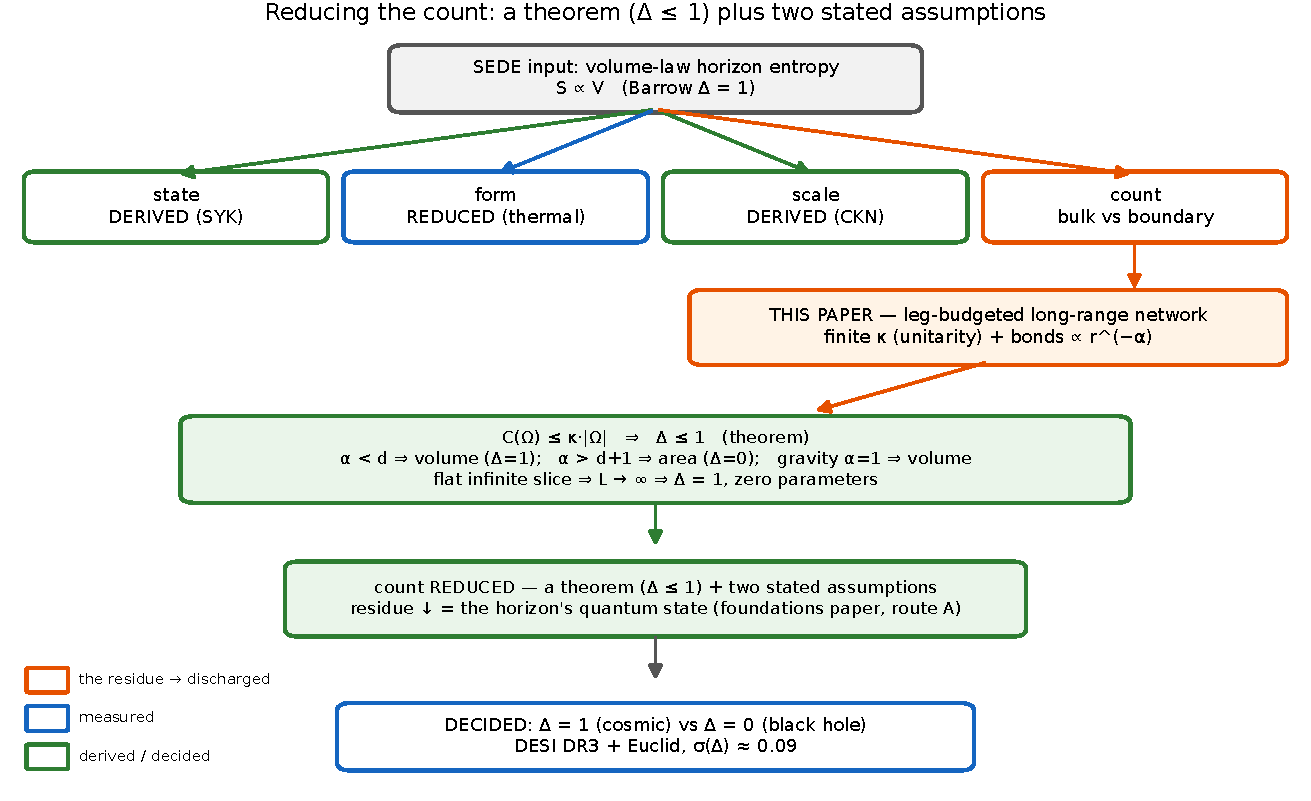
\includegraphics[keepaspectratio]{../../results/count_fig0_reduction}}
\caption{The reduction. SEDE's one input --- volume-law horizon entropy
--- decomposes into \emph{state}, \emph{form}, \emph{scale}, and
\emph{count} (the foundations paper); the first three reduce to
established physics, and the \emph{count} is the irreducible residue.
Modelling the horizon degrees of freedom as a leg-budgeted long-range
network reduces it:
\(C(\Omega ) \leq \kappa \cdot\)\textbar{}\(\Omega\)\textbar{} makes
\(\Delta \leq 1\) a theorem (§\ref{sec-2-2}), \(\alpha < d\) puts
gravity on the volume branch (§\ref{sec-2-3}--§\ref{sec-4}), and
\(\Delta = 1\) is the L → ∞ endpoint of the flat infinite slice --- a
cutoff choice, not a derivation (§\ref{sec-5}). What survives is the
horizon's quantum \emph{state} (route A of the foundations paper) and
that endpoint identification, decided --- with the black-hole
\(\Delta = 0\) --- by DESI DR3 + Euclid.}\label{fig:1}
\end{figure}

\begin{center}\rule{0.5\linewidth}{0.5pt}\end{center}

\section{The count from a leg-budgeted long-range network}\label{sec-2}

\subsection{Setup}\label{sec-2-1}

Let the horizon degrees of freedom be sites of a network filling a ball
of radius L at number density \(n = \ell _{\mathrm{P}}^{-d}\), d = 3,
with symmetric bond weights

\[w_{ij} \propto r_{ij}^{-\alpha}, \qquad \sum_j w_{ij} = \kappa \quad\text{for every } i. \tag{2.1}\]

The budget in (2.1) is not an idealisation. In a tensor-network
representation the leg weight attached to a site is ln(local
Hilbert-space dimension); unitarity bounds it. Given the shape
\(r^{-\alpha }\), the budget is imposed by the unique symmetric scaling
w = diag(d) W diag(d) with prescribed row sums --- the symmetric
Sinkhorn problem, which for positive symmetric W has a unique positive
solution. All numbers below are computed at Sinkhorn residual
\(< 10^{-9}\).

We take as the count the \textbf{bond-cut capacity} of a region
\(\Omega\),

\[C(\Omega) = \sum_{i\in\Omega,\, j\notin\Omega} w_{ij}, \tag{2.2}\]

the standard upper bound on the entanglement entropy of \(\Omega\) with
its complement. C is a capacity, not an entropy: whether it is attained
depends on the state (§\ref{sec-6}). Everything in this section concerns
C.

\subsection{The capacity theorem}\label{sec-2-2}

From (2.1) and (2.2), for any region \(\Omega\),

\[C(\Omega) \le \sum_{i\in\Omega} \sum_j w_{ij} = \kappa\,|\Omega|. \tag{2.3}\]

The entropy of a region cannot exceed its degree-of-freedom count.
Writing \(S \propto  R^{2+\Delta }\) in the Barrow parametrisation
\(S = (A/A_{0})^{1+\Delta /2}\), (2.3) gives

\[\Delta \le 1. \tag{2.4}\]

This is the ceiling of the cosmology paper (§8.1)
\citep{Pandev:2026cosmology} --- obtained here without reference to the
Hausdorff dimension of the horizon, and without the premise that the
horizon is a fractal 2-surface. Finite local dimension is the whole
content. The theorem is model-conditional: it is a statement about the
leg-budgeted network of §\ref{sec-2-1} --- with the \(\alpha  = d\)
crossover of §\ref{sec-2-3} now carrying an explicit finite-size error
bound (Proposition 2.1) rather than an unproven limit interchange ---
not about an arbitrary horizon. Two consequences are worth stating
plainly. First, \(\Delta  > 1\) is impossible in this framework, so a
high-significance measurement of \(\Delta  > 1\) falsifies it with no
parameter available to absorb the result. Second, whatever selects
\(\Delta  = 1\) must be a \emph{saturation} argument, since (2.3) is the
only bound in play.

\subsection{\texorpdfstring{The crossover is at
\(\alpha  = d\)}{The crossover is at \textbackslash alpha  = d}}\label{sec-2-3}

Consider a site at radius s inside a sphere of radius \(\rho  \ll  L\).
The bond mass it places at separations in {[}u, u+du{]} scales as
\(u^{d-1-\alpha }\) du. Its \textbf{outward fraction} --- the share of
its budget spent on bonds crossing \(\rho\) --- is therefore governed by

\[\int^L u^{d-1-\alpha}\,du \quad\text{versus}\quad \int^\rho u^{d-1-\alpha}\,du. \tag{2.5}\]

For \(\alpha  < d\) the integral is dominated by its upper limit: the
bond mass sits at the largest separations, the outward fraction tends to
unity for every interior site, and

\[C(\rho) \to \kappa\, n\, V(\rho) \qquad \text{(volume law, budget saturated).} \tag{2.6}\]

As stated, (2.6) is a limiting statement, and the limits do not commute:
at fixed ambient size L the outward fraction \emph{decreases} with
\(\rho\) and must vanish as \(\rho\) → L, so ``dominated by the upper
limit'' cannot be read as \(\rho\) → ∞ at fixed L. The following
proposition replaces the limit by an explicit finite-size error, uniform
in the site position, and is what the volume law rests on here.

\begin{quote}
\textbf{Proposition 2.1 (uniform outward-fraction bound).} Let sites of
density \(n = \ell ^{-d}\) fill a ball of radius L, let \(\alpha  < d\),
and let \(f_{\mathrm{out}}(x)\) be the fraction of the budget of a site
at x, \textbar x\textbar{} ≤ \(\rho\), carried by bonds crossing the
sphere of radius \(\rho\). Then for every such x,
\[f_{\rm out}(x) \;\ge\; 1 - K(d,\alpha)\,(\rho/L)^{\,d-\alpha}, \qquad
K(d,\alpha) = \frac{S_{d-1}\,2^{\,d-\alpha}/(d-\alpha)}{c_d\,(1-2^{-d})\,2^{-\alpha}},\]
with \(S_{d-1}\) the unit-sphere surface and \(c_{\mathrm{d}}\) the
unit-ball volume. Consequently
\[\kappa\,n\,V(\rho)\left[1 - K(d,\alpha)(\rho/L)^{d-\alpha}\right] \;\le\; C(\rho) \;\le\; \kappa\,n\,V(\rho). \tag{2.6a}\]

\emph{Proof.} Every point of the interior ball lies within distance
\(2\rho\) of x, so the inward mass is at most n
\(S_{d-1}\)\(∫_{0}^{2\rho }\) \(u^{d-1-\alpha }du = n\)
\(S_{d-1}(2\rho )^{d-\alpha }/(d-\alpha )\), the integral converging at
u = 0 precisely because \(\alpha  < d\). Every point of the outer shell
L/2 \textless{} \textbar y\textbar{} \textless{} L lies within distance
2L of x, so the outward mass is at least n
\(c_{\mathrm{d}}(1-2^{-d})L^{d}\cdot (2L)^{-\alpha }\). Since
\(f_{\mathrm{out}} = 1/(1 + in/out)\)≥ \(1 - in/out\), the ratio of
these two gives the stated K. The upper bound in (2.6a) is the capacity
theorem of §\ref{sec-2-2}. ∎
\end{quote}

Three things follow. First, the volume law is a statement at
\textbf{finite} \((\ell\), \(\rho\), L) with a controlled error, so no
interchange of \(\rho\) → ∞ with the continuum limit is invoked. Second,
the same condition \(\alpha  < d\) that makes the short-distance
integral converge is what makes the discrete-to-continuum replacement
safe: the near-field discrepancy between the lattice sum and the
integral is relatively \(O((\ell /\rho )^{d-\alpha })\), vanishing in
the same regime. Third, the error term makes explicit \emph{why}
\(\Delta  = 1\) exactly is the L → ∞ endpoint of §\ref{sec-5} rather
than a finite-size result --- the deficit is governed by \(\rho /L\),
not by \(\rho\) alone.

The bound is rigorous but its constant is not sharp. Numerically
(\texttt{src/outward\_fraction\_bound.py}, d = 3, L = 200, exact angular
average), the measured capacity deficit follows the predicted power
\((\rho /L)^{d-\alpha }\) with a constant of order unity: at gravity's
\(\alpha  = 1\) the fitted deficit exponent is 2.03 against the
predicted \(d - \alpha  = 2\), with
\(K_{\mathrm{measured}} \approx  0.79\) stable across \(\rho  \in  [5\),
40{]}, while the proved constant is K = 13.7 --- valid, and loose by a
factor \(\approx  17\). The fit degrades as \(\alpha\) → d (at
\(\alpha  = 2.5\) the fitted exponent is 0.79 against a predicted 0.5),
which is expected: there the deficit is no longer small and the leading
term does not yet control the behaviour. For gravity's range the
asymptotics are firmly in their regime.

For \(\alpha  > d\) the integral converges at small u: only a surface
layer of thickness \(O(\ell _{\mathrm{P}})\) contributes, and
\(C(\rho ) \propto  A(\rho )\) (area law). The crossover is at
\(\alpha  = d\) exactly --- the same threshold that separates additive
from non-additive long-range systems (Campa--Dauxois--Ruffo
\citep{Campa:2009jxa}), and the same one at which the hypothesis of the
entanglement area-law theorems (Hastings \citep{Hastings:2007iok};
Brandão--Horodecki \citep{Brandao:2013fpa}) fails.

\textbf{Numerical confirmation (Figure 2).} Spherical reduction with the
exact angular average of \textbar{}\(x-y\)\textbar\^{}\((-\alpha )\),
ambient L = 200, \(\kappa  = 1\). The table gives
\(s(\rho ) \equiv  C(\rho )/N_{\mathrm{in}}\), the capacity per enclosed
degree of freedom, and q from \(C \propto  \rho ^{q}\):

\begin{longtable}[]{@{}
  >{\raggedright\arraybackslash}p{(\linewidth - 12\tabcolsep) * \real{0.1429}}
  >{\raggedright\arraybackslash}p{(\linewidth - 12\tabcolsep) * \real{0.1429}}
  >{\raggedright\arraybackslash}p{(\linewidth - 12\tabcolsep) * \real{0.1429}}
  >{\raggedright\arraybackslash}p{(\linewidth - 12\tabcolsep) * \real{0.1429}}
  >{\raggedright\arraybackslash}p{(\linewidth - 12\tabcolsep) * \real{0.1429}}
  >{\raggedright\arraybackslash}p{(\linewidth - 12\tabcolsep) * \real{0.1429}}
  >{\raggedright\arraybackslash}p{(\linewidth - 12\tabcolsep) * \real{0.1429}}@{}}
\caption{Capacity per enclosed degree of freedom
\(s(\rho ) = C(\rho )/N_{\mathrm{in}}\) and measured capacity exponent q
\((C \propto  \rho ^{q})\) versus bond range \(\alpha\), in the
spherical reduction (L = 200, \(\kappa  = 1\)).}\tabularnewline
\toprule\noalign{}
\begin{minipage}[b]{\linewidth}\raggedright
\(\alpha\)
\end{minipage} & \begin{minipage}[b]{\linewidth}\raggedright
\(\rho =2\)
\end{minipage} & \begin{minipage}[b]{\linewidth}\raggedright
\(\rho =5\)
\end{minipage} & \begin{minipage}[b]{\linewidth}\raggedright
\(\rho =10\)
\end{minipage} & \begin{minipage}[b]{\linewidth}\raggedright
\(\rho =20\)
\end{minipage} & \begin{minipage}[b]{\linewidth}\raggedright
\(\rho =40\)
\end{minipage} & \begin{minipage}[b]{\linewidth}\raggedright
q
\end{minipage} \\
\midrule\noalign{}
\endfirsthead
\toprule\noalign{}
\begin{minipage}[b]{\linewidth}\raggedright
\(\alpha\)
\end{minipage} & \begin{minipage}[b]{\linewidth}\raggedright
\(\rho =2\)
\end{minipage} & \begin{minipage}[b]{\linewidth}\raggedright
\(\rho =5\)
\end{minipage} & \begin{minipage}[b]{\linewidth}\raggedright
\(\rho =10\)
\end{minipage} & \begin{minipage}[b]{\linewidth}\raggedright
\(\rho =20\)
\end{minipage} & \begin{minipage}[b]{\linewidth}\raggedright
\(\rho =40\)
\end{minipage} & \begin{minipage}[b]{\linewidth}\raggedright
q
\end{minipage} \\
\midrule\noalign{}
\endhead
\bottomrule\noalign{}
\endlastfoot
1.0 & 0.9999 & 0.9996 & 0.9983 & 0.9933 & 0.9728 & \textbf{2.99} \\
2.0 & 0.9969 & 0.9873 & 0.9707 & 0.9371 & 0.8690 & 2.96 \\
2.5 & 0.9805 & 0.9375 & 0.8850 & 0.8089 & 0.6994 & 2.89 \\
4.0 & 0.7088 & 0.4156 & 0.2569 & 0.1518 & 0.0863 & 2.30 \\
6.0 & 0.5135 & 0.2206 & 0.1119 & 0.0562 & 0.0281 & \textbf{2.03} \\
\end{longtable}

At \(\alpha  = 6\) the capacity per site halves exactly when \(\rho\)
doubles: \(s \propto  1/\rho\), the area law, to three figures. At
\(\alpha  = 1\) it sits at \(\kappa\) to four decimals: \textbf{every
degree of freedom spends essentially its entire budget outward.} The
volume law is not imposed by a ceiling; it is attained.

The \(\alpha  = 4\) row warrants a word, because its q = 2.30 has not
reached 2 and could be mistaken for a failure to converge. It is not:
\(\alpha  = 4 = d + 1\) is the \emph{marginal} area point, where the
capacity-carrying surface layer has a logarithmic tail,
\(C(\rho ) \propto  \rho ^{2}\cdot ln\) \(\rho\), so the finite-\(\rho\)
exponent is \(q(\rho ) = 2 + O(1/ln\) \(\rho\)) --- inflated above 2 but
\emph{decreasing}, not a stable power. Pushing the ambient size out (L =
1500, \(\rho\) up to 180) settles it with a normalisation-free
diagnostic, \(C(\rho )/\rho ^{2}\): at \(\alpha  = 4\) it rises linearly
in ln \(\rho\) \((slope \approx  2.9 > 0)\), the signature of the
marginal logarithm, whereas at \(\alpha  = 5\) --- just past the
marginal point --- it is flat to 6 \% with q = 2.01, the clean area law.
No \(\alpha\) produces a \emph{stable} exponent between 2 and 3: the
\(\alpha  = 4\) elevation is a marginal logarithm on the area side, and
it sharpens rather than softens the binary dichotomy of §\ref{sec-2-4}.
(For \(d < \alpha  < d + 1\) the same analysis gives a genuine but still
non-volume q → \(3 - (\alpha  - d)\); at \(\alpha  = 3.5\), q climbs
toward 2.5. The volume phase, q = 3, is reached only for
\(\alpha  < d\).)

Identifying the saturated capacity with a constant entropy density,

\[s_0 = \kappa\, n = \kappa/\ell_P^3, \tag{2.7}\]

recovers eq. (2.2) of the cosmology paper \citep{Pandev:2026cosmology},
\(s_{\mathrm{grav}} = s_{0}\), with the constant identified as legs per
Planck cell.

\subsection{The dichotomy is binary --- for a gravitational
horizon}\label{sec-2-4}

Equation (2.6) holds for \textbf{every} \(\alpha  < d\), not merely
\(\alpha  = 1\): the volume phase is a basin, not a knife-edge. The
model therefore never requires the specific form w(r) = 1/r. It requires
only

\[w(r)\ \text{decays slower than}\ r^{-d}. \tag{2.8}\]

Any coupling of gravitational reach satisfies (2.8) with room to spare.
We are careful about what is and is not binary. The capacity exponent is
q = 3 (volume) for \emph{every} \(\alpha  < d\) and q = 2 (area) for
\(\alpha  > d+1\); the intermediate window \(d < \alpha  < d+1\) does
interpolate, \(q = 3 - (\alpha  - d)\), with \(\alpha  = d+1\) the
marginal area case (q → 2 with a logarithm) --- the crossover is a
genuine continuum in \(\alpha\) (§\ref{sec-2-3}), not a two-valued
function. What is binary is the count for a \emph{gravitational}
horizon: gravity is 1/r, so \(\alpha  = 1 \ll  d\), sitting deep in the
volume basin, while the equilibrium/area frameworks are local
(effectively \(\alpha  > d+1\)). An intermediate \(\Delta\) would
require an intermediate-\emph{range} horizon coupling,
\(d < \alpha  < d+1\), for which there is no physical mechanism ---
gravity supplies no such exponent. \textbf{A measured intermediate
\(\Delta\) therefore falsifies the gravitational-network picture --- no
coupling of gravitational reach produces it --- rather than selecting a
tunable exponent.} In particular it closes the door on the
Kardar--Parisi--Zhang branch \((\Delta  \approx  0.61)\) once floated as
a distinguishable alternative in the foundations paper: §2.5 shows there
is no roughening universality class to select in the first place.

\begin{figure}
\centering
\pandocbounded{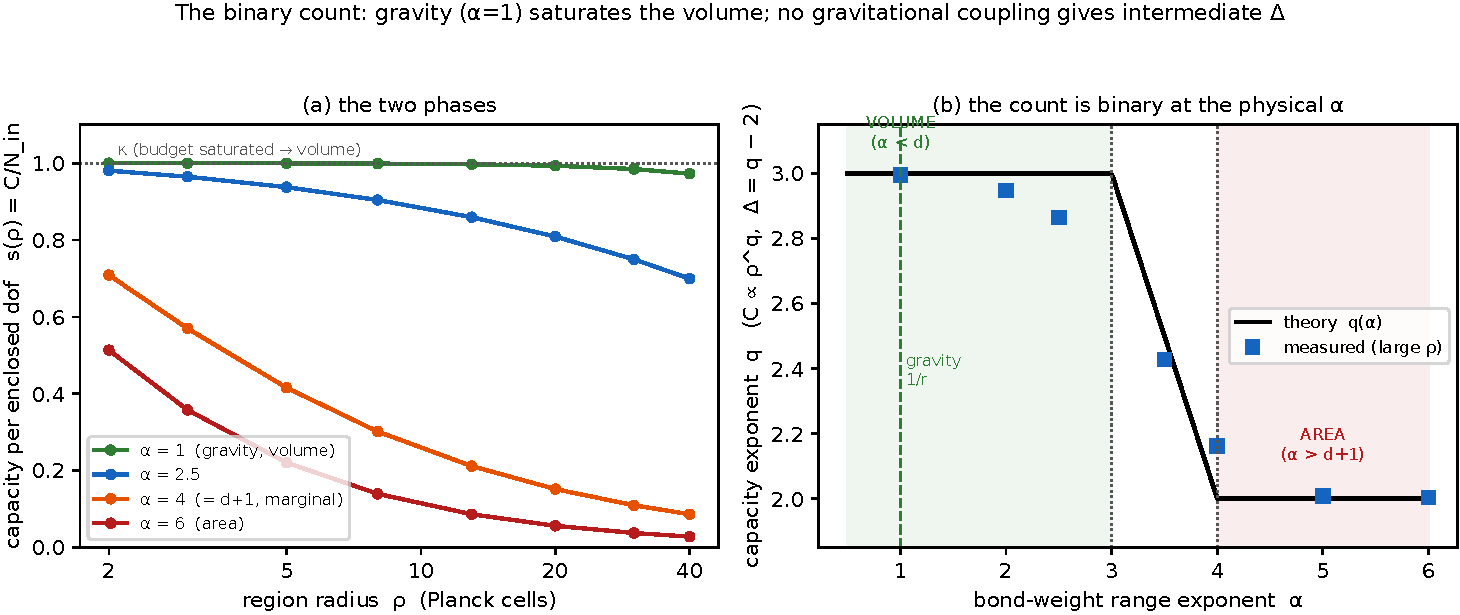
\includegraphics[keepaspectratio]{../../results/count_fig1_dichotomy}}
\caption{The binary count (§\ref{sec-2-3}--2.4). \emph{(a)} Capacity per
enclosed degree of freedom \(s(\rho ) = C/N_{\mathrm{in}}\): at
\(\alpha = 1\) (gravity) it saturates the leg budget \(\kappa\) (the
volume law); at \(\alpha = 6\) it falls as \(1/\rho\) (the area law).
\emph{(b)} The capacity exponent q (with \(\Delta = q - 2\)) versus the
bond-range \(\alpha\): q = 3 (volume) for every \(\alpha < d\) and q = 2
(area) for \(\alpha > d+1\), interpolating only in the \emph{unphysical}
window \(d < \alpha < d+1\) (the marginal \(\alpha = d+1 = 4\) point
carries a logarithm, so its finite-\(\rho\) value sits just above 2).
Gravity's 1/r reach \((\alpha = 1)\) lies deep in the volume basin; no
gravitational coupling yields an intermediate \(\Delta\).}\label{fig:2}
\end{figure}

\subsection{\texorpdfstring{For \(\alpha  < d\) there is no minimum-cut
surface}{For \textbackslash alpha  \textless{} d there is no minimum-cut surface}}\label{sec-2-5}

The Ryu--Takayanagi prescription reads entanglement entropy off a
\emph{minimal cut surface}. That object exists only when the bonds are
local. We test this directly by maximum flow on a lattice ball, with
boundary legs of the upper cap tied to a source and the lower cap to a
sink at infinite capacity, so that every cut passes through the bulk.
Two diagnostics, neither of which depends on any normalisation:

\textbf{(i) Thickness of the severed-bond set, in lattice units}
(weighted RMS of the midpoint height of cut bonds):

\begin{longtable}[]{@{}lllll@{}}
\caption{Thickness of the severed-bond set (weighted RMS midpoint
height, lattice units) versus ball radius R for each bond range
\(\alpha\), from the maximum-flow minimum cut on the lattice
ball.}\tabularnewline
\toprule\noalign{}
\(\alpha\) & R=3 & R=4 & R=5 & R=6 \\
\midrule\noalign{}
\endfirsthead
\toprule\noalign{}
\(\alpha\) & R=3 & R=4 & R=5 & R=6 \\
\midrule\noalign{}
\endhead
\bottomrule\noalign{}
\endlastfoot
0.5 & 0.78 & 1.20 & 1.60 & 1.98 \\
1.0 & 0.82 & 1.27 & 1.70 & 2.11 \\
2.0 & 0.86 & 1.43 & 1.92 & 2.39 \\
3.0 & 0.57 & 1.54 & 2.11 & 2.68 \\
4.0 & 0.55 & 0.59 & 0.63 & 0.64 \\
6.0 & 0.516 & 0.516 & 0.520 & 0.518 \\
\end{longtable}

For \(\alpha  > d\) the thickness is R-independent --- a sharp interface
one lattice spacing thick, and the cut is the equatorial disk
(\textbar S\textbar/N → 0.447, a half-ball). For \(\alpha  \leq  d\) it
grows \(\propto  R\): the severed bonds fill the volume (Figure 3).

\textbf{(ii) Where the cut lives.} For every \(\alpha  \leq  3\) and
every R tested, the fraction of the source side of the minimum cut
consisting of boundary sites is \textbf{1.000, exactly}: the cut
degenerates onto the boundary shell. There is no bulk surface, because
there is no emergent bulk geometry. (The cut cost then scales as
\(R^{5-\alpha }\) --- super-volume --- which is the signature of the
\emph{unbudgeted} network's illegitimacy: per-site leg weight
\(\Sigma _{\mathrm{j}}\) \(r_{\mathrm{ij}}^{-1}\) \textasciitilde{}
\(R^{2}\) diverges, and no finite local Hilbert space supports it.
Imposing (2.1) removes the pathology and returns (2.6).)

\begin{figure}
\centering
\pandocbounded{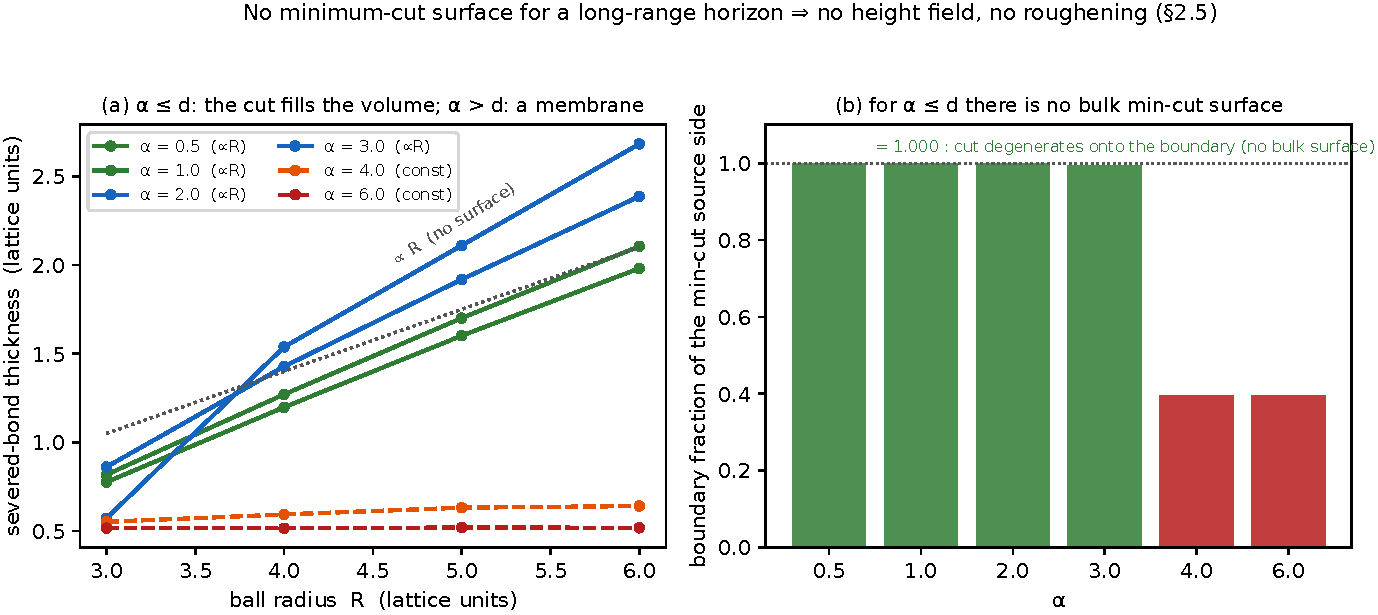
\includegraphics[keepaspectratio]{../../results/count_fig2_membrane}}
\caption{No minimum-cut surface for a long-range horizon
(§\ref{sec-2-5}). \emph{(a)} The thickness of the severed-bond set grows
\(\propto R\) for \(\alpha \leq d\) (the cut fills the volume --- there
is no surface) and is R-independent for \(\alpha > d\) (a one-cell
membrane). \emph{(b)} The boundary fraction of the minimum cut's source
side is 1.000 for \(\alpha \leq d\) (the cut degenerates onto the
boundary shell) and \(\approx 0.40\) for \(\alpha > d\) (a genuine bulk
membrane). With no min-cut surface there is no height field, no
roughness exponent, and no roughening --- so \(\Delta\) is a count, not
a Hausdorff dimension.}\label{fig:3}
\end{figure}

The consequence is structural. With no minimum-cut surface there is no
height field, no roughness exponent, and no roughening universality
class. \textbf{\(\Delta\) is a count, not a Hausdorff dimension},
exactly as the cosmology paper (§8.5) maintains. This is also the
foundations paper's position: it reads the count as the bare bound
\(\Delta  \leq  1\), which §\ref{sec-2-2} here \emph{derives} --- so the
fractal reading \(\Delta  = d_{\mathrm{H}} - 2\) is
unnecessary.\footnote{The \(\epsilon\)-lag / roughening observable of
  the companion papers is superseded here: eq. (2.9) leaves the
  classical apparent horizon with no growth equation to roughen with.
  The companion papers already reflect this --- the foundations paper
  reduces its membrane section to the exact coefficients and withdraws
  the roughening layer, and the cosmology paper withdraws the
  corresponding predictions (its §\ref{sec-6}).}

An independent confirmation from the classical side: in linearised GR
the apparent-horizon condition \(\theta\)₊ = 0 is, in Newtonian gauge
(where the constant-time slicing is shear-free, so \(K_{\mathrm{ij}}\)
is pure trace), the constant-mean-curvature condition
\(\mathcal{M}  = 2H\). It is the Euler--Lagrange equation of
\(A[h] - 2H\cdot V[h]\), and since the area functional A =
R̄²\(∫d\Omega [(1+h)^{2}\)+½\textbar{}\(\nabla _{\mathrm{S}}\) h\textbar²
+ O(\textbar{}\(\nabla _{\mathrm{S}}\) h\textbar⁴){]} carries no cubic
term, the constraint reads

\[\nabla_S^2 h + 2h + 2h^2 = 2\mathcal{S}, \qquad \mathcal{S} = \Phi + \Psi + \dot\Psi/H - H^{-1}\partial_R \Psi. \tag{2.9}\]

There is no \((\nabla h)^{2}\) term at second order, and --- decisively
--- no \(\partial _{\mathrm{t}}\) h at any order. The operator
\(\nabla ^{2}_{\mathrm{S}} + 2\) is elliptic on the sphere;
\(h_\ell m = 2\mathcal{S} _\ell m/(2 - \ell (\ell +1))\) is slaved
instantaneously to the matter perturbations, and high multipoles are
suppressed as \(1/\ell ^{2}\). The classical apparent horizon does not
roughen. It has no growth equation to roughen with. That the
apparent-horizon shape can be found this way --- perturbatively, order
by order, as a slaved constraint within the canonical formalism --- is
independently established by Neuser and Thiemann, who compute it to
second order in gauge-invariant perturbation theory
\citep{Neuser:2026unc}.

This operator is not ours to invent: \(\nabla ^{2}_{\mathrm{S}} + 2\) is
the Andersson--Mars--Simon marginally-outer-trapped-surface (MOTS)
stability operator \citep{Andersson:2007fh} specialised to the FRW
apparent horizon. On the round 2-sphere (areal radius R̄ = 1/H) the AMS
operator L \(\psi  = -\nabla ^{2}_{\mathrm{S}}\) \(\psi  + 2\) \(s^{A}\)
\(D_{\mathrm{A}}\)
\(\psi  + (\)½\(R_{\mathrm{S}}\)−\textbar{}\(\sigma ^{+}\)\textbar² −
\(s_{\mathrm{A}}\) \(s^{A}\)+ \(D_{\mathrm{A}}\) \(s^{A} - 8\pi\)
\(T_{ab}\ell ^{a}\) \(k^{b})\psi\) collapses --- spherical symmetry
gives \(s_{\mathrm{A}} = 0\), the horizon is shear-free
\((\sigma ^{+} = 0)\), and for the within-slice shape variation it
reduces to the classical mean-curvature Jacobi operator
\(-(\nabla ^{2}_{\mathrm{S}}\)+\textbar A\textbar²) with
\textbar A\textbar² = 2/R̄², i.e.~exactly
\(-(1/R\)̄)\((\nabla ^{2}_{\mathrm{S}} + 2)\). Its spectrum is the
published one, ℓ\((\ell +1) - 2\), and the \textbf{ℓ = 1 kernel is the
translation zero mode every MOTS stability operator carries} --- not a
coincidence but the sphere's freedom to be displaced. We reproduce this
independently, by a second geometric route (surface-of-revolution
principal curvatures) matched to the spectrum, so the GR leg of this
argument rests on a published 2008 theorem rather than on our own
symbolic algebra (\texttt{src/ams\_stability.py}).

\emph{Slicing caveat.} The clean \emph{elliptic}
\((\partial _{\mathrm{t}}\)-free) form is specific to the shear-free
Newtonian slice with flat spatial sections. The AMS matter term for FRW
is \(8\pi\) \(T_{ab}\ell ^{a}\) \(k^{b} = 3H^{2}\)+Ḣ, so the
\emph{null-direction} (marginally-outer-trapped-tube,
i.e.~time-evolution) variation carries an Ḣ that the within-slice shape
operator does not: the two differ by exactly the horizon's evolution
term. It is the within-slice shape equation --- the one governing
whether the horizon \emph{roughens} --- that is elliptic and slaved; the
\(\partial _{\mathrm{t}}\) enters only the orthogonal question of how
the horizon moves between slices.

\begin{center}\rule{0.5\linewidth}{0.5pt}\end{center}

\section{\texorpdfstring{The premise: finite local dimension, and why
\(\alpha  < d\) evades the area
law}{The premise: finite local dimension, and why \textbackslash alpha  \textless{} d evades the area law}}\label{sec-3}

The two ingredients of §\ref{sec-2} --- a finite leg budget \(\kappa\)
and a bond weight decaying slower than \(r^{-d}\) --- are not exotic;
each is weaker than something already standard.

\textbf{Finite \(\kappa\) is unitarity.} In a tensor-network
representation of the horizon state, the weight on a leg attached to a
site is the logarithm of the local bond dimension, ln \(\chi\), which a
finite-dimensional local Hilbert space bounds. The per-site budget
\(\Sigma _{\mathrm{j}}\) \(w_{\mathrm{ij}} = \kappa\) of (2.1) is
therefore the statement that each horizon degree of freedom has a
bounded amount of entanglement to distribute --- a consequence of
unitarity, not an assumption about geometry. The bond cut \(C(\Omega )\)
is then the standard Ryu--Takayanagi / minimum-cut upper bound on the
entanglement entropy of \(\Omega\) (§\ref{sec-6-1}). Everything in
§\ref{sec-2-2}--§\ref{sec-2-4} uses only this budget and the
\emph{range} of the weights; it never uses the specific form 1/r.

\textbf{Why \(\alpha  < d\) is allowed --- the area-law theorems and
their hypothesis.} A natural objection is that entanglement entropy
``always'' obeys an area law, so a volume-law horizon is forbidden. It
is not: the entanglement area-law \emph{theorems} are theorems about
\emph{local} systems. In one dimension, gapped local Hamiltonians have
area-law (there, constant) ground-state entanglement
\citep{Hastings:2007iok}; the higher-dimensional results
\citep{Brandao:2013fpa} likewise assume short-range interactions and a
spectral gap. Their load-bearing hypothesis is exactly locality ---
couplings that fall off fast enough that a region's boundary dominates
its entanglement --- and that hypothesis fails precisely when the
weights decay slower than \(r^{-d}\): the same \(\alpha  = d\) threshold
at which our capacity crossover sits (§\ref{sec-2-3}) and at which
long-range statistical mechanics stops being additive
\citep{Campa:2009jxa}. A volume-law entanglement entropy is thus not a
violation of anything; it is the generic expectation once the
connectivity is long-range. The premise (2.8) is the \emph{negation} of
the area-law theorems' hypothesis, and the horizon --- connected by
gravity --- is on the far side of it.

The reduction is therefore in the \emph{strength} of what is assumed.
The postulate replaced was ``the horizon entropy counts its volume.''
What remains is ``the horizon degrees of freedom have finite local
dimension and a longer-than-marginal-range coupling,'' plus the state
assumption of §\ref{sec-6-1}. The first is unitarity; the second is an
inequality gravity satisfies with two decades of margin (§\ref{sec-4});
only the third is a genuine physical input, and it is the foundations
paper's, not ours.

\section{Gravity lands in the volume phase}\label{sec-4}

Which side of the \(\alpha  = d\) crossover is the cosmic horizon on?
The bond weights of (2.1) encode which horizon degrees of freedom are
entangled with which, and how strongly, as a function of separation. For
a horizon whose microscopic correlations are set by gravity, that reach
is Newtonian, \(w(r) \propto  1/r\), so \(\alpha  = 1\) --- well below d
= 3, deep in the volume basin (2.6), with a margin of two full units in
the exponent. This is why the dichotomy of §\ref{sec-2-4} is not
delicate for the physical case: gravity does not sit near the crossover,
and no O(1) uncertainty in the effective coupling could carry it across
two decades to the area side.

That same long-rangedness is the object the foundations paper works with
from the thermodynamic direction. There the horizon degrees of freedom
carry a cooperative coupling
\(J = \lambda _{\mathrm{max}}(W_{\mathrm{grav}})\) --- the largest
eigenvalue of the very weight matrix
\(W_{\mathrm{ij}} \propto  r^{-\alpha }\) of (2.1) --- and
\(\alpha  < d\) is exactly the regime in which that coupling is
\emph{super-extensive}
\((\lambda _{\mathrm{max}} \propto  N^{1-\alpha /d})\) and mean-field
thermodynamics is exact \citep{Campa:2009jxa}. So the network's
``\(\alpha  < d\) ⇒ volume'' of the present paper (the \emph{count}) and
the foundations paper's ``non-additive cooperativity ⇒ a bistable
area↔volume free energy F(m), selected at the horizon's birth'' (the
\emph{selection}) are two readings of one fact: gravity is long-range at
the horizon. The count fixes that the two branches are exactly \{area,
volume\} and that \(\Delta  \leq  1\); the selection fixes which branch
a given horizon occupies --- the grown cosmic horizon carried through
the ordering bifurcation onto the volume branch (a \emph{tilted}
pitchfork, whose absence of branch ambiguity is the generic feature of
its universal unfolding \citep{Golubitsky:1985}), the abruptly-formed
black hole locked on the area branch. The two papers meet here: this one
fixes the ceiling and the two available branches of the count, the
foundations paper the dynamics that selects between them.

\begin{center}\rule{0.5\linewidth}{0.5pt}\end{center}

\section{The edge correction and the infrared cutoff}\label{sec-5}

\subsection{The exact deficit law}\label{sec-5-1}

Equation (2.6) is exact only for \(\rho  \ll  L\). At finite \(\rho /L\)
the outward fraction falls short, because the bond mass a site can place
beyond \(\rho\) is limited by the ambient size. From (2.5), for
\(\alpha  < d\),

\[1 - s(\rho)/\kappa = D(x) = c\, x^{d-\alpha}, \qquad x \equiv \rho/L. \tag{5.1}\]

At \(\alpha  = 1\) no short-distance regulator is needed: Newton's
theorem gives the exact angular average
⟨\textbar{}\(x-y\)\textbar\^{}\((-1)\)⟩ = 1/max(s,s′), and D(x) is a
pure number. Solving the Sinkhorn problem in the radial reduction and
refining the discretisation:

\begin{longtable}[]{@{}lll@{}}
\caption{Convergence of the deficit coefficient \(D(x)/x^{2}\) with the
radial discretisation M, at \(\alpha  = 1\) (exact Newton-kernel angular
average).}\tabularnewline
\toprule\noalign{}
M & \(D(0.02)/x^{2}\) & \(D(0.03)/x^{2}\) \\
\midrule\noalign{}
\endfirsthead
\toprule\noalign{}
M & \(D(0.02)/x^{2}\) & \(D(0.03)/x^{2}\) \\
\midrule\noalign{}
\endhead
\bottomrule\noalign{}
\endlastfoot
750 & 0.6738 & 0.6439 \\
1500 & 0.6732 & 0.6732 \\
3000 & 0.67308 & 0.67316 \\
6000 & 0.67305 & 0.67315 \\
\end{longtable}

\[c = \lim_{x\to0} \frac{D(x)}{x^2} = 0.6730 \pm 0.0001,\]

with a fitted exponent 2.0018 (predicted \(d - \alpha  = 2\)). (Note
that \(D/x^{2}\) drifts upward with x --- 0.6731 at x = 0.02, 0.6817 at
x = 0.20 --- so c must be read as the small-x limit, not as the
intercept of a power-law fit over a finite window.)

The exponent \(d - \alpha\) is confirmed independently at
\(\alpha  = 2\) \((deficit \propto  x)\) and \(\alpha  = 2.5\) \((\)∝
\(x^{1/2}\)). We record that c is \emph{not} 2/3 = 0.66667, from which
it differs by 1\%, well outside the discretisation error. We know of no
closed form and do not assert one.

\subsection{The effective deformation}\label{sec-5-2}

With \(S(\rho ) = \kappa\) n \(V(\rho )[1 - D(\rho /L)]\),

\[\Delta(x) = \frac{d\ln S}{d\ln\rho} - 2 = 1 - \frac{x\, D'(x)}{1 - D(x)} = 1 - \frac{(d-\alpha)\, c\, x^{d-\alpha}}{1 - c\, x^{d-\alpha}}. \tag{5.2}\]

At \(\alpha  = 1\) (Figure 4):

\begin{longtable}[]{@{}lll@{}}
\caption{Effective deformation \(\Delta\) versus the ratio of horizon
radius to network infrared cutoff, \(R_{\mathrm{H}}/L\), at
\(\alpha  = 1\) (eq. 5.2).}\tabularnewline
\toprule\noalign{}
\(R_{\mathrm{H}} / L\) & \(\Delta\) & \\
\midrule\noalign{}
\endfirsthead
\toprule\noalign{}
\(R_{\mathrm{H}} / L\) & \(\Delta\) & \\
\midrule\noalign{}
\endhead
\bottomrule\noalign{}
\endlastfoot
0.001 & 1.0000 & network far exceeds the horizon \\
0.10 & 0.9864 & L = 10 \(R_{\mathrm{H}}\) \\
0.3125 & 0.8546 & L = comoving particle horizon \\
0.50 & 0.5522 & L = 2 \(R_{\mathrm{H}}\) \\
\end{longtable}

The deficit is one-signed: \(D \geq  0\) by (2.3), so the correction
always pushes \(\Delta\) \emph{downward}, toward the area law, and never
above the ceiling. This is consistent with, and is the mechanism behind,
(2.4).

\begin{figure}
\centering
\pandocbounded{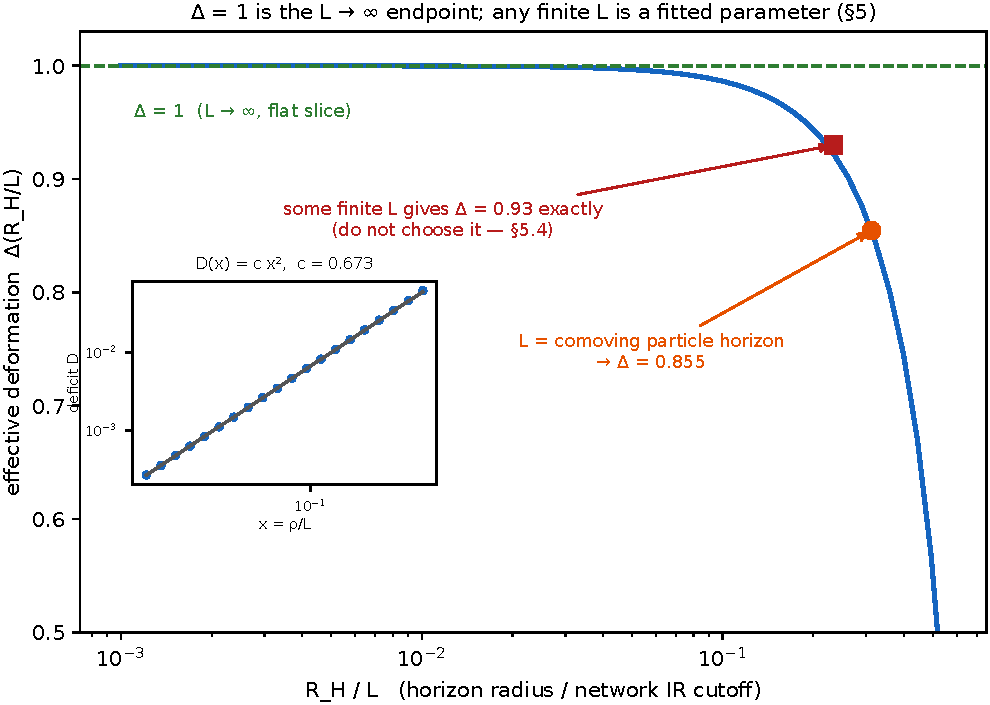
\includegraphics[keepaspectratio]{../../results/count_fig3_cutoff}}
\caption{\(\Delta = 1\) and the infrared cutoff (§\ref{sec-5}). The
effective deformation \(\Delta (R_{\mathrm{H}}/L)\) rises to 1 as the
network cutoff L → ∞. Nothing in the model fixes L, so any finite value
is a fitted dark-sector parameter --- and choosing one is choosing the
answer: L = the comoving particle horizon returns \(\Delta = 0.855\),
and some L reproduces the foundations paper's profile value 0.93 exactly
(§\ref{sec-5-4} cautions against both). Identifying the flat, infinite
spatial slice with the network cutoff takes L → ∞ and \(\Delta = 1\) ---
the endpoint choice of §\ref{sec-5-3}, which eliminates the parameter
without deriving the value. Inset: the exact deficit law
\(D(x) = c\cdot x^{2}\) at \(\alpha = 1\) (Newton kernel), c =
0.673.}\label{fig:4}
\end{figure}

\subsection{L is not fixed by the model}\label{sec-5-3}

Expression (5.2) is a one-parameter family in L. Nothing in SEDE --- not
the CKN bound, not flatness, not the structure gate, not the
birth-selection chain of the foundations paper's §5 --- determines the
infrared cutoff of the horizon's degree-of-freedom network. Adopting any
finite L therefore introduces a continuously-sampled dark-sector
parameter, which is precisely what the model's central claim forbids
(the cosmology paper's §3: \emph{the dark sector adds no fitted
parameter}).

The only value of L consistent with the model's own background is L → ∞.
The spatial slice of flat FRW is infinite; its flatness is already used,
in the cosmology paper's §2, to normalise \(\Omega _\mathrm{DE}0\). With
L → ∞, D → 0 and

\[\Delta = 1 \quad\text{exactly.} \tag{5.3}\]

We are explicit about the status of this step, because it is where the
value of \(\Delta\) actually enters. The argument above eliminates the
would-be parameter; it does not derive its value. The step that fixes L
is the identification of the cosmological spatial slice with the
infrared cutoff of the entanglement network --- an identification
nothing in SEDE determines. \(\Delta  = 1\) is therefore the
\emph{endpoint reading}: a cutoff choice made for consistency with the
model's own no-fitted-parameter claim, under which the pre-registered
point carries no free parameter --- and it remains the theory's one
postulate, restated, not a theorem of this counting. (An earlier version
of this paper presented \(\Delta  = 1\) as ``exact, with zero free
parameters,'' full stop; that phrasing conflated eliminating a parameter
by a cutoff choice with deriving its value, and is corrected
throughout.) The point value \textbf{agrees with the foundations paper}:
an earlier \(\Delta  \in  [0.98\), 1{]} window there, whose derivation
rested on a logarithmic Edwards--Wilkinson roughening of the horizon
surface, collapses to the point \(\Delta  = 1\) once that roughening is
removed --- as it is both there and in §\ref{sec-2-5} here. This paper
now grounds that point value in the network capacity, as the L → ∞
endpoint. There was never a window that is both derived and free.

\subsection{A warning we place in the text deliberately}\label{sec-5-4}

Setting L equal to the comoving particle horizon \((\)≈ 3.2
\(R_{\mathrm{H}}\)) returns \(\Delta  = 0.855\). The profile-likelihood
interval of the foundations paper's §7 is \(\Delta  = 0.93\) {[}0.83,
1.02{]}. There exists a choice of L returning 0.93 exactly.

We do not make it, and we recommend that no one does. A prediction is
over-determined only when every quantity entering it is fixed
independently of the datum it is compared against. Here the only
principle available fixes \(L = \infty\) and hence \(\Delta  = 1\); any
other value of L is selected by the answer. The same discipline applies
to a second numerical coincidence in this programme: the volume well of
the foundations paper's free energy sits at m* ≈ 0.93, and m is an
amplitude while \(\Delta\) is an exponent. Two coincidences at the same
value, neither carrying information.

\subsection{Pre-registration}\label{sec-5-5}

\begin{longtable}[]{@{}
  >{\raggedright\arraybackslash}p{(\linewidth - 4\tabcolsep) * \real{0.3333}}
  >{\raggedright\arraybackslash}p{(\linewidth - 4\tabcolsep) * \real{0.3333}}
  >{\raggedright\arraybackslash}p{(\linewidth - 4\tabcolsep) * \real{0.3333}}@{}}
\caption{Pre-registered predictions for the Barrow deformation
\(\Delta\) and the conditions under which the framework is
falsified.}\tabularnewline
\toprule\noalign{}
\begin{minipage}[b]{\linewidth}\raggedright
statement
\end{minipage} & \begin{minipage}[b]{\linewidth}\raggedright
value
\end{minipage} & \begin{minipage}[b]{\linewidth}\raggedright
status
\end{minipage} \\
\midrule\noalign{}
\endfirsthead
\toprule\noalign{}
\begin{minipage}[b]{\linewidth}\raggedright
statement
\end{minipage} & \begin{minipage}[b]{\linewidth}\raggedright
value
\end{minipage} & \begin{minipage}[b]{\linewidth}\raggedright
status
\end{minipage} \\
\midrule\noalign{}
\endhead
\bottomrule\noalign{}
\endlastfoot
driven cosmic horizon & \(\Delta  = 1\) exactly & pre-registered point;
the L → ∞ endpoint reading (a postulate, §\ref{sec-5-3}), no free
parameter once the endpoint is adopted \\
equilibrium horizon (black hole) & \(\Delta  = 0\) & the foundations
paper's §5(iii), unchanged \\
intermediate \(\Delta\) & not produced by any gravitational (1/r,
\(\alpha <d\)) or local coupling & \textbf{falsifies the framework}
(§\ref{sec-2-4}) \\
\(\Delta  > 1\) & impossible & \textbf{falsifies the framework}
(§\ref{sec-2-2}) \\
\end{longtable}

DESI DR3 + Euclid reach a forecast \(\sigma (\Delta ) \approx  0.09\)
(Fisher, hence optimistic): \(\Delta  = 1\) separates from
\(\Delta  = 0\) at a nominal \textasciitilde{}\(11\sigma\) and from any
intermediate value at \(\gtrsim  4\sigma\).

\begin{center}\rule{0.5\linewidth}{0.5pt}\end{center}

\section{From capacity to entropy: the state factor and the
gate}\label{sec-6}

Everything in §\ref{sec-2} concerns the \emph{capacity} \(C(\Omega )\)
--- the bond-cut upper bound on the entanglement entropy of a region.
Turning a capacity into the horizon entropy S that enters the cosmology
(the cosmology paper's \(\rho _\mathrm{DE} = T_\mathrm{AH}\)
\(s_{\mathrm{grav}}\)) takes one further ingredient, and it is worth
isolating exactly what it is and what it is not.

\subsection{Attainment is the state question}\label{sec-6-1}

The bond cut \(C(\Omega ) = \Sigma _{i\in \Omega , j\notin \Omega }\)
\(w_{\mathrm{ij}}\) is the Ryu--Takayanagi/minimum-cut \emph{bound}:
\(S(\Omega ) \leq  C(\Omega )\), with equality only for a state that
saturates it. So the whole of §\ref{sec-2} --- the theorem
\(\Delta  \leq  1\), the \{area, volume\} dichotomy, the \(\alpha  = d\)
crossover --- is state-\emph{independent}; but the identification
\textbf{S = C}, which fixes the \emph{value} of the entropy rather than
its scaling, is not. It holds when the horizon degrees of freedom are
maximally entangled (thermalised, Page-saturated), so that every bond
across the cut carries its full ln \(\chi\). That is precisely the
\emph{state} half of the postulate, argued independently in the
foundations paper (route A: Sachdev--Ye--Kitaev (SYK) / maximal
scrambling) and untouched here. We are explicit that this is the one
thing §\ref{sec-2} does not remove: the network fixes the \emph{count}
--- which degrees of freedom a region's entropy may draw on --- while
the maximally-scrambled state fixes that they are all in fact used.
§\ref{sec-2} makes the count a theorem; the value of the entropy still
rests on the state.

\textbf{The saturating state is not exotic: it is the tracial state of
the site algebra.} The assumption can be sharpened from ``some state
saturates every cut'' to an identification internal to the model. Each
site carries a finite Hilbert dimension \(e^{\kappa }\), so the site
algebra of a region \(\Omega\) is a finite-dimensional factor with dim
𝓗\_\(\Omega  = e^{\kappa |\Omega |}\). Its maximally mixed (tracial)
state assigns
\[S(\Omega) \;=\; \log \dim \mathcal{H}_\Omega \;=\; \kappa|\Omega| \qquad \text{for \emph{every} } \Omega,\]
i.e.~it attains the capacity bound of §\ref{sec-2-2} identically, region
by region --- not as a fine-tuned configuration but as the
maximum-entropy state of the very algebra whose capacity §\ref{sec-2}
bounds. The ``cut-saturating state'' and the ``maximally scrambled
state'' are therefore the same object described from two sides, and S =
C holds in it by construction.

Two qualifications keep this honest. First, saturation of \emph{every}
cut requires the global state to be mixed: a pure state obeys
\(S(\Omega ) = S(\Omega ^{c})\) and is capped by
\(min(\kappa\)\textbar{}\(\Omega\)\textbar,
\(\kappa\)\textbar{}\(\Omega ^{c}\)\textbar), so it cannot saturate both
a region and its complement. For a horizon-bounded region mixedness is
the physical situation --- the exterior purifies the interior --- and it
is also the situation in the crossed-product description, whose
maximal-entropy state is likewise maximally mixed. Second, this
identifies the saturating state; it does not prove that a given
\emph{physical} horizon is in it. What it removes is the suspicion that
the saturating state is a special construction invented to reach
\(\Delta  = 1\): it is the flat state of the model's own algebra, and
the remaining question --- whether horizon dynamics drives the state to
it --- is the scrambling question already stated, not an additional one.

\subsection{The entropy density and the occupancy gate}\label{sec-6-2}

On the volume branch \((\alpha  < d)\) with the saturating state,
\(S(\rho ) = C(\rho ) = \kappa\) n \(V(\rho )\), so the entropy density
is the constant

\[s_0 = \kappa n = \kappa/\ell_P^3 \tag{6.1}\]

of eq. (2.7) --- the cosmology paper's \(s_{\mathrm{grav}}\), legs per
Planck cell. A horizon does not, however, carry its full volume capacity
at every epoch: the capacity is \emph{populated} as structure drives it.
Writing \(f_{\mathrm{sat}} \in  [0\), 1{]} for the activated fraction,

\[S = f_{\rm sat}\, s_0\, V, \tag{6.2}\]

the driven limit \(f_{\mathrm{sat}}\) → 1 is the volume law
\((\Delta  = 1)\) and the undriven limit \(f_{\mathrm{sat}}\) → 0 is the
area baseline \((\Delta  = 0)\) --- the state-dependent count of the
foundations paper's §7.1, now with \(s_{0}\) supplied by the network
rather than posited. The gate is not a new function: minimal absorption
kinetics --- each deposit activates a fraction of the \emph{remaining}
inactive capacity, df \(= \gamma (1 - f)\) \(d(D^{2})\) --- integrate to
\(f_{\mathrm{sat}} = 1 - e^{-\gamma  D^{2}}\), exactly the cosmology
paper's gate (the foundations paper's §7.1a).

\subsection{Occupancy is not the order parameter (a correction to Fig. 3
of the foundations paper)}\label{sec-6-3}

It is tempting to identify \(f_{\mathrm{sat}}\) with the order parameter
m of the area↔volume free energy F(m) of the foundations paper's §5.
They are different variables, and their dynamics part company at the
endpoint. The order parameter is a \emph{free-energy} coordinate: it
relaxes by gradient flow, \(\partial _\tau\) \(m = -\Gamma\) F′(m), a
branch-\emph{selecting} dynamics fixed by the shape of F and driven by
the pitchfork at the horizon's birth. The occupancy is a
\emph{cumulative} coordinate: it obeys the gate kinetics
\(\partial _{\mathrm{x}}\) \(f = \gamma (1 - f)\) (§\ref{sec-6-2}),
whose rate \textbf{vanishes as f → 1} --- a monotone filling that can
never overshoot and carries no barrier. A variable whose own equation of
motion switches off at the endpoint it is approaching cannot be the
order parameter of a double-well potential. The division of labour is
therefore clean: the \emph{branch} --- which well the horizon sits in
--- is fixed at birth by m (the foundations paper's §5 iii);
\(f_{\mathrm{sat}}\) is the subsequent \emph{occupancy} of the
already-selected volume capacity, not a second branch selector. Insofar
as the presentation of Fig. 3 of the foundations paper invites its
landscape to be read against \(f_{\mathrm{sat}}\), the landscape
variable is the order parameter m; \(f_{\mathrm{sat}}\) is the distinct
occupancy coordinate of (6.2).

\subsection{The loop to the cosmology paper}\label{sec-6-4}

Equations (6.1)--(6.2) close the chain from the count to the observable
with no fitted dark-sector parameter. The entropy density
\(s_{0} = \kappa n\) is fixed by unitarity (legs per Planck cell); the
exponent \(\Delta  = 1\) by §\ref{sec-2} (the volume branch) and
§\ref{sec-5} (the flat slice, L → ∞ --- the endpoint choice); the gate
\(f_{\mathrm{sat}}\) by the derived kinetics of §\ref{sec-6-2}. These
are exactly the two dark-sector inputs the cosmology paper's
horizon-fluid ansatz \(\rho _\mathrm{DE} = T_\mathrm{AH}\)
\(s_{\mathrm{grav}}\) requires --- the volume-law entropy density and
its occupancy --- so the cosmology paper's background is reproduced with
every dark-sector quantity now grounded in the network count. What is
\emph{not} discharged, and we say so plainly, is the state assumption of
§\ref{sec-6-1}: §\ref{sec-2} makes the ceiling and the dichotomy
theorems, but the value of the horizon entropy is attained only for the
maximally-scrambled state carried over from the foundations paper. That
single assumption is the honest residue of the capacity→entropy step.

\begin{center}\rule{0.5\linewidth}{0.5pt}\end{center}

\section{The residue}\label{sec-7}

\begin{longtable}[]{@{}
  >{\raggedright\arraybackslash}p{(\linewidth - 4\tabcolsep) * \real{0.3333}}
  >{\raggedright\arraybackslash}p{(\linewidth - 4\tabcolsep) * \real{0.3333}}
  >{\raggedright\arraybackslash}p{(\linewidth - 4\tabcolsep) * \real{0.3333}}@{}}
\caption{The assumption ledger: status of each component of the
volume-law input before this paper (the foundations paper's §8) and
after the reduction.}\tabularnewline
\toprule\noalign{}
\begin{minipage}[b]{\linewidth}\raggedright
item
\end{minipage} & \begin{minipage}[b]{\linewidth}\raggedright
status before (the foundations paper's §8)
\end{minipage} & \begin{minipage}[b]{\linewidth}\raggedright
status now
\end{minipage} \\
\midrule\noalign{}
\endfirsthead
\toprule\noalign{}
\begin{minipage}[b]{\linewidth}\raggedright
item
\end{minipage} & \begin{minipage}[b]{\linewidth}\raggedright
status before (the foundations paper's §8)
\end{minipage} & \begin{minipage}[b]{\linewidth}\raggedright
status now
\end{minipage} \\
\midrule\noalign{}
\endhead
\bottomrule\noalign{}
\endlastfoot
state (maximal entanglement) & first-principles (route A / SYK) &
unchanged \\
form \((S \propto  V)\) & reduces to thermalisation & unchanged \\
scale \((\rho _\mathrm{DE}\) ∼ \(\rho _{\mathrm{crit}}\)) & CKN bound +
flatness & unchanged \\
\textbf{count (bulk vs boundary)} & \textbf{open --- the residue} &
\textbf{reduced (§\ref{sec-2}, §\ref{sec-5}): binary \{0, 1\} given the
network model; \(\Delta  = 1\) is the L → ∞ endpoint choice, still a
postulate} \\
geometric ceiling \(\Delta  \leq  1\) & postulate in effective form
(cosmology paper, §8.1); reduced to bound-only in the foundations paper,
§7.1 & theorem (2.3)--(2.4) \\
\(\Delta  = d_{\mathrm{H}} - 2\) (fractal horizon) & assumed (cosmology
paper, §8.1); withdrawn in the foundations paper & \textbf{withdrawn}
(§\ref{sec-2-5}) \\
roughening class (EW vs KPZ) & conditional prediction (foundations
paper, pre-fold) & \textbf{no such classification exists} \\
transverse diffusivity coefficient & scoped open coefficient
(foundations paper, §5 iv) & \textbf{not defined} (§\ref{sec-2-5}); the
\(\epsilon\)-lag layer it fed is retracted in the foundations paper
(§\ref{sec-6}) \\
--- & --- & \emph{new:} finite leg budget \(\kappa\) (unitarity) \\
--- & --- & \emph{new:} w(r) decays slower than \(r^{-d}\) \\
--- & --- & \emph{new:} the horizon dof are a network \\
--- & --- & \emph{new:} the infinite-cutoff identification L → ∞
(§\ref{sec-5-3}) \\
\end{longtable}

Four premises remain, and they are weaker than the one they replace. The
leg budget is unitarity. The bond-weight condition is an inequality, not
a functional form, and gravity satisfies it with two decades of margin
in the exponent. The infrared-cutoff identification is a stated endpoint
choice --- the residue of the original postulate, relocated and made
explicit rather than eliminated (§\ref{sec-5-3}). The state premise is
untouched and independently argued. What has gone is the
bulk-versus-boundary count \emph{as a free binary} --- the item both
previous papers name as irreducible is now a binary forced to \{0, 1\}
by the network's range dichotomy --- together with the fractal reading
of \(\Delta\) and the roughening layer built on it.

We claim a reduction, not a proof. The bond cut is a capacity, an upper
bound on entanglement entropy; its attainment is the state question, and
the identification of the horizon degrees of freedom with a network of
the assumed connectivity is a model of the horizon, not a derivation of
one. What the reduction buys is that the remaining conditionality now
sits in one place, is stated as an inequality, and is decided --- for
the one horizon we have --- by a measurement already scheduled.

\begin{center}\rule{0.5\linewidth}{0.5pt}\end{center}

\section{Discussion}\label{sec-8}

\textbf{Status: this is a complexity/connectivity layer, not a proven
entropy derivation (governing note).} Read the construction below as a
model of coarse-grained horizon \emph{connectivity}, decoupled from any
claim to have derived a gravitational entropy or a stress tensor. Three
points govern. \textbf{(i)} The volume-scaling quantity is a structural
\textbf{complexity} \(C_{\rm str}\), not the generalized entropy
\(S_{\rm gen}\): the bond-cut capacity bounds how many degrees of
freedom a region's entropy \emph{draws on}, which need not equal
\(A/4G + S_{\rm out}\). \textbf{(ii)} A horizon-tracking CKN cutoff
gives an \emph{area-like} \(\Delta = 0\) (density \(\propto H^2\)), not
the volume-like \(\Delta = 1\); the volume count is the
\emph{non-default} identification, allowed by long-rangedness
(\(\alpha < d\)) but not forced, and the one concrete de Sitter model
(double-scaled SYK) currently reads as area --- so \(\Delta = 1\)
remains the empirical bet of the cosmology paper, tested by DESI DR3 +
Euclid, not a theorem of this counting. \textbf{(iii)} The bridge to
cosmology is an \emph{empirical ansatz}, not a derivation:
\[C_{\rm str}\ \longrightarrow\ q_R = \sigma_R^2\ \longrightarrow\ u(q_R),\]
i.e.~the complexity is identified with the model-owned filtered matter
variance \(q_R = \sigma_R^2\) (R = 8 \(h^{-1}Mpc\)) that gates the
FPAB-SEDE background --- and its ensemble and renormalization are
\emph{not} specified here. We do \textbf{not} infer the cosmological
amplitude \(\mu\), the filter scale R, the normalization \(q_*\) or the
braiding fraction \(b\) from node counting; those are fixed by the
finite cubic-KGB action and the data (the cosmology paper), and all
cosmological comparisons below should be read against that action's
predictions, not the earlier smooth-fluid solution.

\textbf{The de Sitter holography question, addressed constructively.}
The residue lives in de Sitter holography \citep{Strominger:2001pn}. The
foundations paper reduced the count to its sharpest form: in the
crossed-product (Type \(\mathrm{II}_{1}\)) description of the de Sitter
static patch, the \emph{value} of the maximal horizon entropy is a trace
calibration --- a free normalisation the algebra does not fix --- so
``the eternal-patch ceiling is the area'' is an Einstein-saddle
calibration, not an algebraic output, and the FRW-patch calibration is
left open as ``the count asked algebraically.'' This paper answers it
constructively, without solving the operator-algebraic problem: the
trace is fixed by the network --- \(\kappa\) legs per Planck cell ---
and the count that trace delivers is \emph{volume}, because the
horizon's connectivity is long-range \((\alpha  < d)\). We do not claim
to have computed dim 𝓗(static patch) non-perturbatively; we claim that
the quantity the \(\mathrm{II}_{1}\) calibration stands in for --- how
many degrees of freedom a horizon region's entropy draws on --- is a
bond count, and that bond count is the enclosed volume for any
gravitational horizon. Consistently with the foundations paper, the
algebra \emph{type} is not the discriminator (an accelerating attractor
is \(\mathrm{II}_{1}\)-compatible either way); the calibration is, and
the calibration is the leg budget.

\textbf{What is not settled.} One thing, stated plainly --- the list is
shorter than in earlier drafts, and we record what moved. The
\(\alpha  = d\) crossover of §\ref{sec-2-3} previously rested on a
dominance argument that was correct term by term but interchanged the
\(\rho\) → ∞ and continuum limits without justification; Proposition 2.1
now replaces that interchange with a two-sided bound at finite
\((\ell\), \(\rho\), L), uniform in the site position, whose error term
is explicitly \(O((\rho /L)^{d-\alpha })\) and is verified numerically.
The derivation gap is closed; what remains there is only that the proved
constant is not sharp (loose by ≈ 17 at \(\alpha  = 1\)), which affects
no conclusion. What is \emph{not} settled is the identification S = C,
the state question (§\ref{sec-6-1}): the network gives the count, the
maximally-scrambled state gives that the count is attained. That
assumption is route A of the foundations paper, and it is the honest
residue of the whole programme --- now a single question, and one shared
with area-law black holes (a black hole carries the same
maximally-entangled horizon state; what differs is that it is undriven,
so its capacity is the boundary count, §\ref{sec-6-2}). The open content
of SEDE is thereby relocated, in its entirety, from the \emph{count} to
the \emph{state}. That state question is itself now narrower than it
was: §\ref{sec-6-1} identifies the saturating state as the tracial state
of the site algebra --- the flat state of the model's own algebra, which
attains the capacity bound for every region identically --- so what
remains is not ``does a saturating state exist'' but ``is a physical
horizon driven to it,'' which is the scrambling / Page-curve question
the foundations paper takes up. We do not claim that last step is closed
here.

\textbf{Falsifiability.} Because the count is discrete for a
gravitational horizon (§\ref{sec-2-4}), the prediction is a
\emph{point}, \(\Delta  = 1\), not a fitted exponent: an intermediate
\(\Delta\) is not a universality class to be selected but a refutation,
and DESI DR3 + Euclid forecast \(\sigma (\Delta ) \approx  0.09\)
(Fisher) --- separating volume from area at a nominal
\textasciitilde{}\(11\sigma\) and from any intermediate value at
\(\gtrsim  4\sigma\). The companion black-hole channel \((\Delta  = 0\)
for equilibrium horizons, §\ref{sec-6-2}) makes the framework
falsifiable on a \emph{second}, independent horizon: an isolated
volume-law black hole would mean the deformation is universal, refuting
the state-dependent, driven-versus-equilibrium count. Resting the count
on a network makes SEDE more falsifiable, not less.

\section{Conclusion}\label{sec-9}

We set out to reduce the one input the foundations paper could not ---
whether the cosmic horizon's entropy counts its enclosed bulk or its
boundary. Modelling the horizon degrees of freedom as a network with a
finite leg budget and long-range bonds, we found the \emph{ceiling} is a
theorem and the count binary: the bond-cut capacity bounds
\(\Delta  \leq  1\) identically; the capacity is the enclosed volume for
every coupling of range \(\alpha  < d\) and the boundary area for
\(\alpha  > d+1\), with gravity's 1/r reach \((\alpha  = 1)\) deep on
the volume side. The value \(\Delta  = 1\) is not a theorem of this
counting: it is the L → ∞ endpoint of the one free scale --- the
infrared cutoff, which nothing internal fixes --- reached by identifying
the flat, infinite spatial slice with the network cutoff, a stated
choice under which the pre-registered point carries no free parameter.
The fractal reading of \(\Delta\) is unnecessary (the ceiling is a
finite-dimension bound) and, we showed, unavailable (no minimum-cut
surface exists for a long-range network, hence no Hausdorff dimension
and no roughening) --- which retires, across the companion papers, the
roughening layer once built on it. What remains is strictly weaker than
the postulate it replaces: finite local dimension, a range inequality
gravity satisfies with room to spare, the infinite-cutoff
identification, and a maximally-scrambled state. The last two are the
residue --- a \emph{state} question and an \emph{endpoint} choice, no
longer a free counting --- the same questions area-law black holes now
answer, and the same measurement, \(\Delta\) to a forecast
\(\sigma  \approx  0.09\) at DESI DR3 + Euclid, that decides them for
the one horizon we have.

\begin{center}\rule{0.5\linewidth}{0.5pt}\end{center}

\section*{Reproducibility}\label{reproducibility}
\addcontentsline{toc}{section}{Reproducibility}

Every number above is produced by the accompanying code from a single
entry point, with validation assertions at each stage:

\begin{itemize}
\tightlist
\item
  \texttt{src/mincut\_membrane.py} --- maximum-flow minimum cut on the
  lattice ball; membrane-thickness and shell-fraction diagnostics
  (§\ref{sec-2-5}, tables i--ii).
\item
  \texttt{src/capacity\_radial.py} --- spherical reduction with the
  exact angular average; the \(\alpha\)-crossover table of
  §\ref{sec-2-3} and the large-\(\rho\) \(C(\rho )/\rho ^{2}\)
  diagnostic (marginal-log at \(\alpha  = d + 1\) vs clean area at
  \(\alpha  > d + 1\)), asserted.
\item
  \texttt{src/outward\_fraction\_bound.py} --- the finite-size
  outward-fraction bound of Proposition 2.1: fits the capacity-deficit
  exponent against the predicted \(d - \alpha\) and checks every
  measured deficit against the proved bound \(K(\rho /L)^{d-\alpha }\),
  asserted.
\item
  \texttt{src/edge\_deficit.py} --- Newton-kernel solve at
  \(\alpha  = 1\); the deficit law and the convergence of c
  (§\ref{sec-5-1}).
\item
  \texttt{src/horizon\_constraint.py} --- symbolic expansion of the
  apparent-horizon condition, eq. (2.9); verified against the exact mean
  curvature of a translated sphere.
\item
  \texttt{src/ams\_stability.py} --- external-standard check: eq. (2.9)
  is the Andersson--Mars--Simon MOTS stability operator on the FRW round
  sphere. Independent (surface-of-revolution) derivation of
  −(1/R̄)\((\nabla ^{2}_{\mathrm{S}} + 2)\), the published spectrum
  ℓ\((\ell +1) - 2\) with the ℓ = 1 translation zero mode, and the AMS
  matter term \(8\pi\) \(T_{ab}\ell ^{a}\) \(k^{b} = 3H^{2}\)+Ḣ that
  isolates the slicing caveat.
\item
  \texttt{run\_all.py} --- single entry point; runs every stage with
  validation assertions.
\item
  \texttt{figures/make\_figures.py} --- regenerates the four figures
  from the same \texttt{src/} computations (Figs 1--4 →
  \texttt{output/count\_fig\{0–3\}\_*.png}).
\end{itemize}

\begin{center}\rule{0.5\linewidth}{0.5pt}\end{center}

\section*{Data availability
statement}\label{data-availability-statement}
\addcontentsline{toc}{section}{Data availability statement}

The code that supports the findings of this article is openly available
at \url{https://github.com/spsingularity/sede-count}, with a tagged
release archived at Zenodo, DOI
\href{https://doi.org/10.5281/zenodo.21525523}{10.5281/zenodo.21525523}.
Every quantitative claim is reproduced from a single entry point
(\texttt{run\_all.py}, also wired into the repository-wide
\texttt{reproduce\_all.py} as the \texttt{netcount} stage), each stage
carrying validation assertions that all pass, and the four figures
regenerate from the same computations via
\texttt{figures/make\_figures.py}. No observational data were generated
or analysed beyond the standard public inputs cited in the companion
papers.

\section*{Funding}\label{funding}
\addcontentsline{toc}{section}{Funding}

This research received no external funding.

\section*{Competing interests}\label{competing-interests}
\addcontentsline{toc}{section}{Competing interests}

The author, an independent researcher, declares no competing interests.

\section*{Ethics statement}\label{ethics-statement}
\addcontentsline{toc}{section}{Ethics statement}

Not applicable. This work is purely theoretical and involved no human
participants, human data or tissue, and no animal subjects.

\section*{Acknowledgements}\label{acknowledgements}
\addcontentsline{toc}{section}{Acknowledgements}

As sole author, S. Pandev conceived and carried out the study, performed
and independently verified all analyses, and wrote the manuscript,
taking full responsibility for its content. Artificial-intelligence
tools --- Claude Opus 4.x (Anthropic) --- assisted with drafting and
editing the manuscript, developing and cross-checking the analysis code,
and literature searches; all output, including every literature
reference, was checked by the author, who takes full responsibility for
the content. No AI tool is an author.
\bibliographystyle{iopart-num}
\bibliography{refs,refs_foundations}
\end{document}
